% Options for packages loaded elsewhere
\PassOptionsToPackage{unicode}{hyperref}
\PassOptionsToPackage{hyphens}{url}
\PassOptionsToPackage{dvipsnames,svgnames,x11names}{xcolor}
%
\documentclass[
  letterpaper,
  DIV=11,
  numbers=noendperiod]{scrartcl}
\usepackage{amsmath,amssymb}
\usepackage{lmodern}
\usepackage{iftex}
\ifPDFTeX
  \usepackage[T1]{fontenc}
  \usepackage[utf8]{inputenc}
  \usepackage{textcomp} % provide euro and other symbols
\else % if luatex or xetex
  \usepackage{unicode-math}
  \defaultfontfeatures{Scale=MatchLowercase}
  \defaultfontfeatures[\rmfamily]{Ligatures=TeX,Scale=1}
\fi
% Use upquote if available, for straight quotes in verbatim environments
\IfFileExists{upquote.sty}{\usepackage{upquote}}{}
\IfFileExists{microtype.sty}{% use microtype if available
  \usepackage[]{microtype}
  \UseMicrotypeSet[protrusion]{basicmath} % disable protrusion for tt fonts
}{}
\makeatletter
\@ifundefined{KOMAClassName}{% if non-KOMA class
  \IfFileExists{parskip.sty}{%
    \usepackage{parskip}
  }{% else
    \setlength{\parindent}{0pt}
    \setlength{\parskip}{6pt plus 2pt minus 1pt}}
}{% if KOMA class
  \KOMAoptions{parskip=half}}
\makeatother
\usepackage{xcolor}
\IfFileExists{xurl.sty}{\usepackage{xurl}}{} % add URL line breaks if available
\IfFileExists{bookmark.sty}{\usepackage{bookmark}}{\usepackage{hyperref}}
\hypersetup{
  colorlinks=true,
  linkcolor={blue},
  filecolor={Maroon},
  citecolor={Blue},
  urlcolor={Blue},
  pdfcreator={LaTeX via pandoc}}
\urlstyle{same} % disable monospaced font for URLs
\usepackage{longtable,booktabs,array}
\usepackage{calc} % for calculating minipage widths
% Correct order of tables after \paragraph or \subparagraph
\usepackage{etoolbox}
\makeatletter
\patchcmd\longtable{\par}{\if@noskipsec\mbox{}\fi\par}{}{}
\makeatother
% Allow footnotes in longtable head/foot
\IfFileExists{footnotehyper.sty}{\usepackage{footnotehyper}}{\usepackage{footnote}}
\makesavenoteenv{longtable}
\usepackage{graphicx}
\makeatletter
\def\maxwidth{\ifdim\Gin@nat@width>\linewidth\linewidth\else\Gin@nat@width\fi}
\def\maxheight{\ifdim\Gin@nat@height>\textheight\textheight\else\Gin@nat@height\fi}
\makeatother
% Scale images if necessary, so that they will not overflow the page
% margins by default, and it is still possible to overwrite the defaults
% using explicit options in \includegraphics[width, height, ...]{}
\setkeys{Gin}{width=\maxwidth,height=\maxheight,keepaspectratio}
% Set default figure placement to htbp
\makeatletter
\def\fps@figure{htbp}
\makeatother
\setlength{\emergencystretch}{3em} % prevent overfull lines
\providecommand{\tightlist}{%
  \setlength{\itemsep}{0pt}\setlength{\parskip}{0pt}}
\setcounter{secnumdepth}{-\maxdimen} % remove section numbering
\KOMAoption{captions}{tableheading}
\makeatletter
\makeatother
\makeatletter
\@ifpackageloaded{caption}{}{\usepackage{caption}}
\AtBeginDocument{%
\renewcommand*\contentsname{Table of contents}
\renewcommand*\listfigurename{List of Figures}
\renewcommand*\listtablename{List of Tables}
\renewcommand*\figurename{Figure}
\renewcommand*\tablename{Table}
}
\@ifpackageloaded{float}{}{\usepackage{float}}
\floatstyle{ruled}
\@ifundefined{c@chapter}{\newfloat{codelisting}{h}{lop}}{\newfloat{codelisting}{h}{lop}[chapter]}
\floatname{codelisting}{Listing}
\newcommand*\listoflistings{\listof{codelisting}{List of Listings}}
\makeatother
\makeatletter
\@ifpackageloaded{caption}{}{\usepackage{caption}}
\@ifpackageloaded{subcaption}{}{\usepackage{subcaption}}
\makeatother
\makeatletter
\makeatother
\ifLuaTeX
  \usepackage{selnolig}  % disable illegal ligatures
\fi

\author{}
\date{}

\begin{document}

\hypertarget{sec-intro}{%
\section{Introduction}\label{sec-intro}}

In section Section~\ref{sec-intro}

\hypertarget{sec-method}{%
\section{Methodological background}\label{sec-method}}

Counterfactual search happens in the feature space: we are interested in
understanding how we need to change individual attributes in order to
change the model output to a desired value or label
(\cite{molnar2020interpretable}). Typically the underlying methodology
is presented in the context of binary classification:
\(M: \mathcal{X} \mapsto y\) where and \(y\in\{0,1\}\). Let \(t=1\) be
the target class and let \(\overline{x}\) denote the factual feature
vector of some individual outside of the target class, so
\(\overline{y}=M(\overline{x})=0\). We follow this convention here,
though it should be noted that the ideas presented here also carry over
to multi-class problems and regression (\cite{molnar2020interpretable}).

\hypertarget{generic-framework}{%
\subsection{Generic framework}\label{generic-framework}}

Then the counterfactual search objective originally proposed by
\cite{wachter2017counterfactual} is as follows

\begin{equation}\protect\hypertarget{eq-obj}{}{
\min_{\underline{x} \in \mathcal{X}} h(\underline{x}) \ \ \ \mbox{s. t.} \ \ \ M(\underline{x}) = t
}\label{eq-obj}\end{equation}

where \(h(\cdot)\) quantifies how complex or costly it is to go from the
factual \(\overline{x}\) to the counterfactual \(\underline{x}\). To
simplify things we can restate this constrained objective
(Equation~\ref{eq-obj}) as the following unconstrained and
differentiable problem:

\begin{equation}\protect\hypertarget{eq-solution}{}{
\underline{x} = \arg \min_{\underline{x}}  \ell(M(\underline{x}),t) + \lambda h(\underline{x})
}\label{eq-solution}\end{equation}

Here \(\ell\) denotes some loss function targeting the deviation between
the target label and the predicted label and \(\lambda\) governs the
stength of the complexity penalty. Provided we have gradient access for
the black-box model \(M\) the solution to this problem
(Equation~\ref{eq-solution}) can be found through gradient descent. This
generic framework lays the foundation for most state-of-the-art
approaches to counterfactual search and is also used as the baseline
approach - \texttt{GenericGenerator} - in our package. The
hyperparameter \(\lambda\) is typically tuned through grid search.
Conventional choices for \(\ell\) include margin-based losses like
cross-entropy loss and hinge loss. It is worth pointing out that the
loss function is typically computed with respect to logits rather than
predicted probabilities, a convetion that we have chosen to
follow.\footnote{While the rationale for this convention is not entirely
  obvious, implementations of loss functions with respect to logits are
  often numerically more stable. For example, the
  \texttt{logitbinarycrossentropy(ŷ,\ y)} implementation in
  \texttt{Flux.Losses} (used here) is more stable than the
  mathematically equivalent \texttt{binarycrossentropy(ŷ,\ y)}.}

Numerous - and in some cases competing - extensions to this simple
approach have been developed since counterfactual explanations were
first proposed in 2017 (see \cite{verma2020counterfactual} and
\cite{karimi2020survey} for surveys). The various approaches largely
differ in how they define the complexity penalty. In
\cite{wachter2017counterfactual}, for example, \(h(\cdot)\) is defined
in terms of the Manhattan distance between factual and counterfactual
feature values. While this is an intuitive choice, it is too simple to
address many of the desirable properties of effective counterfactual
explanations that have been set out. These desiderata include:
\textbf{closeness} - the average distance between factual and
counterfactual features should be small
(\cite{wachter2017counterfactual}); \textbf{actionability} - the
proposed feature perturbation should actually be actionable
(\cite{ustun2019actionable}, \cite{poyiadzi2020face});
\textbf{plausibility} - the counterfactual explanation should be
plausible to a human (\cite{joshi2019towards}); \textbf{unambiguity} - a
human should have no trouble assigning a label to the counterfactual
(\cite{schut2021generating}); \textbf{sparsity} - the counterfactual
explanation should involve as few individual feature changes as possible
(\cite{schut2021generating}); \textbf{robustness} - the counterfactual
explanation should be robust to domain and model shifts
(\cite{upadhyay2021towards}); \textbf{diversity} - ideally multiple
diverse counterfactual explanations should be provided
(\cite{mothilal2020explaining}); and \textbf{causality} - counterfactual
explanations reflect the structual causal model underlying the data
generating process
(\cite{karimi2020algorithmic},\cite{karimi2021algorithmic}).

\hypertarget{counterfactuals-for-bayesian-models}{%
\subsection{Counterfactuals for Bayesian
models}\label{counterfactuals-for-bayesian-models}}

For what follows it is worth elaborating on the approach proposed in
\cite{schut2021generating}. The authors demonstrate that many of the
abovementioned desiderata can be addressed very easily, if the
classifier \(M\) is Bayesian. In particular, they show that close,
realistic, sparse and unambigous counterfactuals can be generated by
implicitly minimizing the classifier's predictive uncertainty through a
greedy counterfactual search. Formally, they define \(h(\cdot)\) as the
predictive entropy of the classifier, which captures both
\textbf{epistemic} and \textbf{aleatoric} uncertainty: the former is
high on points far away from the training data while the latter is high
in regions of the input space that are inherently noisy. Both are
regions we want to steer clear off in our counterfactual search and
hence predictive entropy is an intuitive choice for a complexity
penalty. The authors further point out that any solution that minimizes
cross-entropy loss (Equation~\ref{eq-solution}) also minimizes
predictive entropy:
\(\arg \min _{\underline{x}} \ell(M(\underline{x}),t) \in \arg \min _{\underline{x}} h(\underline{x})\).
Let \(\mathcal{\widetilde{M}}\) denote the class of binary classifiers
that incorporate predictive uncertainty, then the previous observation
implies that the optimal solution to counterfactual search
(Equation~\ref{eq-solution}) can be restated as follows:

\begin{equation}\protect\hypertarget{eq-solution-bayes}{}{
\underline{x} = \arg \min_{\underline{x}}  \ell(M(\underline{x}),t) \ \ , \ \  \forall M\in\mathcal{\widetilde{M}}
}\label{eq-solution-bayes}\end{equation}

We can drop the complexity penalty altogether and still generate
effective counterfactual explanations. As we will see below, even a fast
and greedy counterfactual search proposed in \cite{schut2021generating}
yields good results in this setting. The approach has been implemented
as \texttt{GreedyGenerator} in our package and should only be used with
classifiers of type \(\mathcal{\widetilde{M}}\). It is worth noting that
the findings in \cite{schut2021generating} are not mutually exclusive of
many of the other methodologies that have been put foward. On the
contrary, we believe that they are complementary: the generic
counterfactual search proposed in \cite{wachter2017counterfactual}, for
example, can be shown to produce more plausible counterfactuals in the
Bayesian setting. Similarly, there is no obvious reason why recent work
on diversity (\cite{mothilal2020explaining}), robustness
(\cite{upadhyay2021towards}) and causality
(\cite{karimi2020algorithmic},\cite{karimi2021algorithmic}) could not be
complemented by the findings in \cite{schut2021generating}. For this
reason we are highlighting \cite{schut2021generating} here and have
prioritized it in the development of
\texttt{CounterfactualExplanations}. While there is no free lunch and
\(M\in\mathcal{\widetilde{M}}\) may seem like a hard constraint, recent
advances in probabilistic machine learning have shown that the
computational cost involved in Bayesian model averaging is lower than we
may have thought (\cite{gal2016dropout},
\cite{lakshminarayanan2016simple}, \cite{daxberger2021laplace},
\cite{murphy2022probabilistic}).

\hypertarget{using-counterfactualexplanations}{%
\section{\texorpdfstring{Using
\texttt{CounterfactualExplanations}}{Using CounterfactualExplanations}}\label{using-counterfactualexplanations}}

The package is built around two modules that are designed to be as
scalable as possible through multiple dispatch: 1) \texttt{Models} is
concerned with making any arbitrary model compatible with the package;
2) \texttt{Generators} is used to implement arbitrary counterfactual
search algorithms.\footnote{We have made an effort to keep the code base
  a flexible and scalable as possible, but cannot guarantee at this
  point that really any counterfactual generator can be implemented
  without further adaptation.} The core function of the package
\texttt{generate\_counterfactual} uses an instance of type
\texttt{T\ \textless{}:\ FittedModel} produced by the \texttt{Models}
module (Figure~\ref{fig-models}) and an instance of type
\texttt{T\ \textless{}:\ Generator} produced by the \texttt{Generators}
module (Figure~\ref{fig-generators}). Relating this back the methodology
outlined in Section~\ref{sec-method}, the former instance corresponds to
the model \(M\) while the latter defines the rules for the
counterfactual search (Equation~\ref{eq-solution} and
Equation~\ref{eq-solution-bayes}). In the following we will demonstrate
how to use and extend the package architecture through a few examples.

\begin{figure}

{\centering 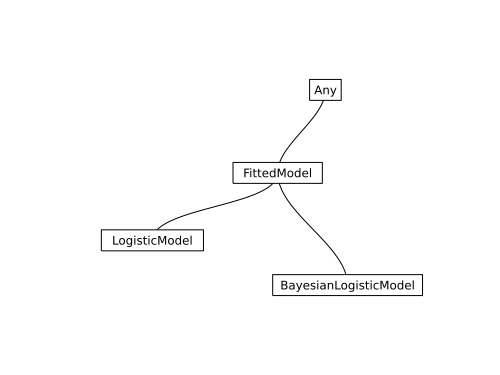
\includegraphics[width=3.33333in,height=2.5in]{www/models.png}

}

\caption{\label{fig-models}Schematic overview of the
\texttt{FittedModel} base type and its descendants.}

\end{figure}

\begin{figure}

{\centering 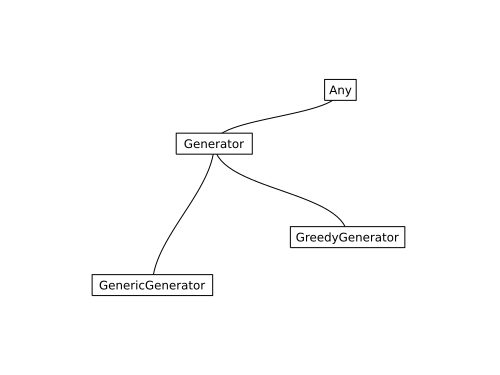
\includegraphics[width=3.33333in,height=2.5in]{www/generators.png}

}

\caption{\label{fig-generators}Schematic overview of the
\texttt{Generator} base type and its descendants.}

\end{figure}

\hypertarget{getting-started}{%
\subsection{Getting started}\label{getting-started}}

The code below provides a complete example demonstrating how the
framework presented in Section~\ref{sec-method} can be implemeted in
Julia using the \texttt{CounterfactualExplantions} package: using a
synthetic data set with linearly separable samples we firstly define our
model and then generate a counterfactual for a randomly selected sample.
Figure~\ref{fig-binary} shows the resulting counterfactual path in the
two-dimensional feature space: features go through iterative
perturbations until the desired confidence level is reached as
illustrated by the contour in the background, which indicates the
classifier's predicted probability that the label is equal to 1.

It may help to go through the relevants parts of the code in some more
detail starting from the part involving the model. For illustrative
purposes the \texttt{Models} module ships with a constructor for a
logistic regression model:
\texttt{LogisticModel(W::Matrix,b::AbstractArray)\ \textless{}:\ FittedModel}.
This constructors does not fit the regression model, but rather takes
its underlying parameters as given. In other words, it is generally
assumed that the user has already estimated a model. Based on the
provided estimates two functions are already implemented that compute
logits and probabilities for the model, respectively. Below we will see
how users can use multiple dispatch to extend these functions for use
with arbitrary models. For now it is enough to note that those methods
define how the model makes its predictions \(M(x)\) and hence they form
an integral part of the counterfactual search.

With the model \(M\) defined in the code below we go on to set up the
counterfactual search as follows: 1) choose a random sample
\texttt{x\_factual}; 2) compute its factual label \texttt{y\_factual} as
predicted by the model (\(M(\overline{x})=0\)); and 3) specify the other
class as our \texttt{target} label (\(t=1\)) along with a desired level
of \texttt{confidence} in the final prediction \(M(\underline{x})=t\).

The last two lines of the code below define the counterfactual generator
and finally run the counterfactual search. The first three fields of the
\texttt{GenericGenerator} are reserved for hyperparameters governing the
strength of the complexity penalty, the step size for gradient descent
and the tolerance for convergence. The fourth field accepts a
\texttt{Symbol} defining the type of loss function \(\ell\) to be used.
Since we are dealing with a binary classification problem logistic
binary cross-entropy is an appropriate choice.\footnote{As mentioned
  earlier, the loss function is computed with respect to logits and
  hence it is important to use logistic binary cross-entropy loss as
  opposed to just binary cross-entropy.} The fifth and last field can be
used to define mutability constraints for the features.

\begin{lstlisting}[language = Julia]
# Data:
using CounterfactualExplanations, Random
Random.seed!(1234);
N = 100 # number of data points
using CounterfactualExplanations.Data
x, y = toy_data_linear(N) 

# Model:
using CounterfactualExplanations.Models 
w = [1.0 1.0]# true coefficients
b = 0
M = LogisticModel(w, [b])

# Setup:
x_factual = x[rand(1:length(x))]
y_factual = round(probs(M, x_factual)[1])
target = ifelse(y_factual==1.0,0.0,1.0) 
confidence = 0.75 

# Counterfactual search:
generator = GenericGenerator(
    0.1,0.1,1e-5,:logitbinarycrossentropy,nothing)
counterfactual = generate_counterfactual(
    generator, x_factual, M, target, confidence)
\end{lstlisting}

\begin{figure}

{\centering 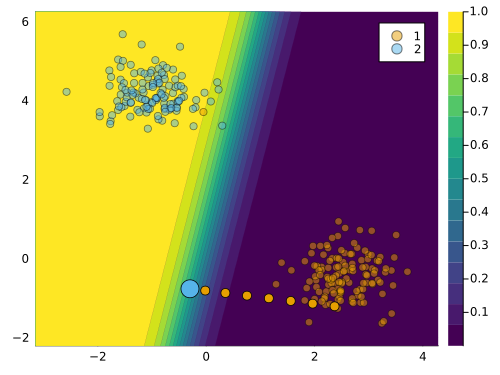
\includegraphics[width=3.33333in,height=2.5in]{www/ce_binary.png}

}

\caption{\label{fig-binary}Counterfactual path using generic
counterfactual generator for conventional binary classifier.}

\end{figure}

In this simple example the generic generator produces an effective
counterfactual: the decision boundary is crossed (i.e.~the
counterfactual explanation is valid) and upon visual inspection the
counterfactual seems plausible (Figure~\ref{fig-binary}). Still, the
example also illustrates that things may well go wrong: since the
underlying model produces high-confidence predictions in regions free of
any data, it is easy to think of scenarios that involve valid but
unrealistic or ambiguous counterfactuals. Consider, for example, the
scenario illustrated in Figure~\ref{fig-binary-wrong}, which involves
the same logisitic classifier albeit massively overfitted. In this case
generic search may yield an unrealistic counterfactual that is well into
the yellow region and yet far away from all other samples (red marker)
or an ambiguous counterfactual near the decision boundary (black
marker).

\begin{figure}

{\centering 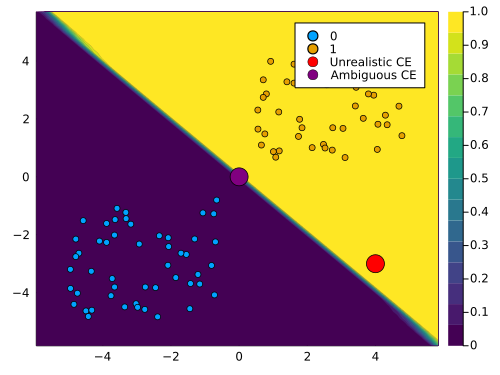
\includegraphics[width=3.33333in,height=2.5in]{www/binary_wrong.png}

}

\caption{\label{fig-binary-wrong}Unrealistic and ambiguous
counterfactuals that may be produced by generic counterfactual search
for an overfitted conventional binary classifier.}

\end{figure}

Among the different approaches that have recently been put forward to
deal with such issues is the greedy generator for Bayesian models
proposed by \cite{schut2021generating}. For reasons discussed in
Section~\ref{sec-method}, we have chosen to prioritize this approach in
the development of \texttt{CounterfactualExplanations}. The code below
shows how this approach can be implemented.

\begin{lstlisting}[language = Julia]
using LinearAlgebra
I = UniformScaling(1)
cov = Symmetric(reshape(randn(9),3,3).*0.01 + I) 
w = [1 1]
params = hcat(b, w)
M = BayesianLogisticModel(params, cov);
generator = GreedyGenerator(
    0.25,20,:logitbinarycrossentropy,nothing)
counterfactual = generate_counterfactual(
    generator, x_factual, M, target, confidence)
\end{lstlisting}

\begin{figure}

{\centering 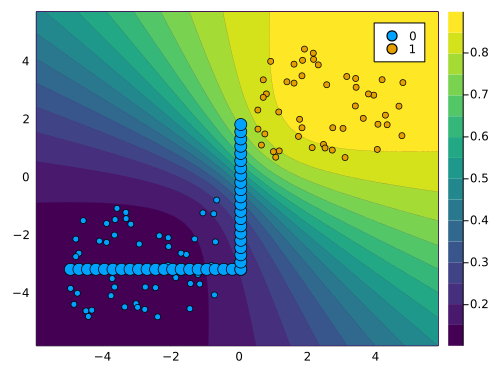
\includegraphics[width=3.33333in,height=2.5in]{www/ce_binary_laplace.png}

}

\caption{\label{fig-binary-laplace}Counterfactual path using greedy
counterfactual generator for Bayesian binary classifier.}

\end{figure}

\hypertarget{custom-models}{%
\subsection{Custom models}\label{custom-models}}

\hypertarget{empirical-example}{%
\section{Empirical example}\label{empirical-example}}

\hypertarget{related-and-future-work}{%
\section{Related and future work}\label{related-and-future-work}}

\end{document}
